\thispagestyle{empty}
\chapter{Análisis de Semejantes}

Tal y como se ha reflejado en la introducción, el proceso a seguir para optener un diseño preliminar, será el análisis de semejantes.
Este análisis consiste en crear una base de datos de aeronaves ya existentes, cuyas características sean similares a las que podría tener la nuestra, de manera que mediante un análisis estadístico se pueda obtener una primera aproximación de algunas características de nuestra aeronave.\\

Dado que el objetivo es el diseño de un helicóptero no tripulado de 450 Kg de \emph{MTOW}, los vehículos a analizar serán helicópteros de una masa similar, en torno a 400-500 kg, pero al no existir una cantidad suficiente dentro de este margen, se ha decidido ampliar este.


% Table generated by Excel2LaTeX from sheet 'Hoja1'
\begin{table}[htbp]
	\centering
	\caption{Add caption}
	\begin{tabular}{|c|r|r|r|r|r|l|r|r|r|r|l|}
		\rowcolor[rgb]{ .22,  .337,  .137} \textcolor[rgb]{ 1,  1,  1}{MODELO} & \multicolumn{1}{c|}{\textcolor[rgb]{ 1,  1,  1}{MTOW(kg)}} & \multicolumn{1}{c|}{\textcolor[rgb]{ 1,  1,  1}{DIAMETRO(m)}} & \multicolumn{1}{c|}{\textcolor[rgb]{ 1,  1,  1}{Omega(rad/s)}} & \multicolumn{1}{c|}{\textcolor[rgb]{ 1,  1,  1}{b}} & \multicolumn{1}{c|}{\textcolor[rgb]{ 1,  1,  1}{btr}} & \multicolumn{1}{c|}{\textcolor[rgb]{ 1,  1,  1}{Motorización}} & \multicolumn{1}{c|}{\textcolor[rgb]{ 1,  1,  1}{Autonomía (horas)}} & \multicolumn{1}{c|}{\textcolor[rgb]{ 1,  1,  1}{Techo(m)}} & \multicolumn{1}{c|}{\textcolor[rgb]{ 1,  1,  1}{Altura(m)}} & \multicolumn{1}{c|}{\textcolor[rgb]{ 1,  1,  1}{Vmáx (km/h)}} & \multicolumn{1}{c|}{\textcolor[rgb]{ 1,  1,  1}{UAV}} \\
		\rowcolor[rgb]{ .329,  .506,  .208} \textcolor[rgb]{ 1,  1,  1}{SA-200 Weasel*} & \cellcolor[rgb]{ .659,  .816,  .553}70 & \cellcolor[rgb]{ .659,  .816,  .553}2,07 & \cellcolor[rgb]{ .659,  .816,  .553}167,55 & \cellcolor[rgb]{ .659,  .816,  .553}2 & \cellcolor[rgb]{ .659,  .816,  .553}6 & \cellcolor[rgb]{ .659,  .816,  .553}jet-turbine & \cellcolor[rgb]{ .659,  .816,  .553}2,5 & \cellcolor[rgb]{ .659,  .816,  .553}3100 & \cellcolor[rgb]{ .659,  .816,  .553}0,95 & \cellcolor[rgb]{ .659,  .816,  .553}167 & \cellcolor[rgb]{ .659,  .816,  .553}TRUE \\
		\midrule
		\rowcolor[rgb]{ .329,  .506,  .208} \textcolor[rgb]{ 1,  1,  1}{Scout B1-100} & \cellcolor[rgb]{ .659,  .816,  .553}77 & \cellcolor[rgb]{ .659,  .816,  .553}3,2 & \cellcolor[rgb]{ 1,  1,  0} & \cellcolor[rgb]{ .659,  .816,  .553}2 & \cellcolor[rgb]{ .659,  .816,  .553}2 & \cellcolor[rgb]{ .659,  .816,  .553}Alternativo & \cellcolor[rgb]{ .659,  .816,  .553}1,5 & \multicolumn{1}{l|}{\cellcolor[rgb]{ .659,  .816,  .553}\newline{}} & \cellcolor[rgb]{ .659,  .816,  .553}1 & \multicolumn{1}{l|}{\cellcolor[rgb]{ 1,  1,  0}\newline{}} & \cellcolor[rgb]{ .659,  .816,  .553}TRUE \\
		\midrule
		\rowcolor[rgb]{ .329,  .506,  .208} \textcolor[rgb]{ 1,  1,  1}{Neo S300} & \cellcolor[rgb]{ .659,  .816,  .553}85 & \cellcolor[rgb]{ .659,  .816,  .553}3 & \cellcolor[rgb]{ 1,  1,  0} & \cellcolor[rgb]{ .659,  .816,  .553}3 & \cellcolor[rgb]{ .659,  .816,  .553}2 & \cellcolor[rgb]{ .659,  .816,  .553}Eléctrico & \cellcolor[rgb]{ 1,  1,  0} & \cellcolor[rgb]{ 1,  1,  0} & \cellcolor[rgb]{ .659,  .816,  .553}0,95 & \cellcolor[rgb]{ 1,  1,  0} & \cellcolor[rgb]{ .659,  .816,  .553}TRUE \\
		\midrule
		\rowcolor[rgb]{ .329,  .506,  .208} \textcolor[rgb]{ 1,  1,  1}{Yamaha R-50*} & \cellcolor[rgb]{ .659,  .816,  .553}90 & \cellcolor[rgb]{ .659,  .816,  .553}3,07 & \cellcolor[rgb]{ .659,  .816,  .553}88,6 & \cellcolor[rgb]{ .659,  .816,  .553}2 & \cellcolor[rgb]{ .659,  .816,  .553}2 & \cellcolor[rgb]{ .659,  .816,  .553}Alternativo & \cellcolor[rgb]{ .659,  .816,  .553}1 & \cellcolor[rgb]{ .659,  .816,  .553}300 & \cellcolor[rgb]{ .659,  .816,  .553}1,08 & \cellcolor[rgb]{ 1,  1,  0} & \cellcolor[rgb]{ .659,  .816,  .553}TRUE \\
		\midrule
		\rowcolor[rgb]{ .329,  .506,  .208} \textcolor[rgb]{ 1,  1,  1}{R-350*} & \cellcolor[rgb]{ .659,  .816,  .553}150 & \cellcolor[rgb]{ .659,  .816,  .553}3,5 & \cellcolor[rgb]{ .659,  .816,  .553}82,86 & \cellcolor[rgb]{ .659,  .816,  .553}3 & \cellcolor[rgb]{ .659,  .816,  .553}2 & \cellcolor[rgb]{ .659,  .816,  .553}jet-turbine & \cellcolor[rgb]{ .659,  .816,  .553}2 & \cellcolor[rgb]{ .659,  .816,  .553}2500 & \cellcolor[rgb]{ .659,  .816,  .553}1,3 & \cellcolor[rgb]{ .659,  .816,  .553}120 & \cellcolor[rgb]{ .659,  .816,  .553}TRUE \\
		\midrule
		\rowcolor[rgb]{ .329,  .506,  .208} \textcolor[rgb]{ 1,  1,  1}{SD 150 Hero*} & \cellcolor[rgb]{ .659,  .816,  .553}150 & \cellcolor[rgb]{ .659,  .816,  .553}3,5 & \cellcolor[rgb]{ .659,  .816,  .553}105,14 & \cellcolor[rgb]{ .659,  .816,  .553}3 & \cellcolor[rgb]{ .659,  .816,  .553}2 & \cellcolor[rgb]{ .659,  .816,  .553}jet-turbine & \cellcolor[rgb]{ .659,  .816,  .553}5 & \cellcolor[rgb]{ .659,  .816,  .553}4000 & \cellcolor[rgb]{ .659,  .816,  .553}1,2 & \cellcolor[rgb]{ .659,  .816,  .553}90 & \cellcolor[rgb]{ .659,  .816,  .553}TRUE \\
		\midrule
		\rowcolor[rgb]{ .329,  .506,  .208} \textcolor[rgb]{ 1,  1,  1}{APID 55*} & \cellcolor[rgb]{ .659,  .816,  .553}160 & \cellcolor[rgb]{ .659,  .816,  .553}3,3 & \cellcolor[rgb]{ .659,  .816,  .553}54,54 & \cellcolor[rgb]{ .659,  .816,  .553}2 & \cellcolor[rgb]{ .659,  .816,  .553}2 & \cellcolor[rgb]{ .659,  .816,  .553}Alternativo & \cellcolor[rgb]{ .659,  .816,  .553}4,5 & \cellcolor[rgb]{ .659,  .816,  .553}3000 & \cellcolor[rgb]{ .659,  .816,  .553}1,2 & \cellcolor[rgb]{ .659,  .816,  .553}90 & \cellcolor[rgb]{ .659,  .816,  .553}TRUE \\
		\midrule
		\rowcolor[rgb]{ .329,  .506,  .208} \textcolor[rgb]{ 1,  1,  1}{APID 60*} & \cellcolor[rgb]{ .659,  .816,  .553}180 & \cellcolor[rgb]{ .659,  .816,  .553}3,3 & \cellcolor[rgb]{ .659,  .816,  .553}90,97 & \cellcolor[rgb]{ .659,  .816,  .553}2 & \cellcolor[rgb]{ .659,  .816,  .553}2 & \cellcolor[rgb]{ .659,  .816,  .553}Alternativo & \cellcolor[rgb]{ .659,  .816,  .553}4,5 & \cellcolor[rgb]{ .659,  .816,  .553}3000 & \cellcolor[rgb]{ .659,  .816,  .553}1,2 & \cellcolor[rgb]{ .659,  .816,  .553}110 & \cellcolor[rgb]{ .659,  .816,  .553}TRUE \\
		\midrule
		\rowcolor[rgb]{ .329,  .506,  .208} \textcolor[rgb]{ 1,  1,  1}{Camcopter S100*} & \cellcolor[rgb]{ .659,  .816,  .553}200 & \cellcolor[rgb]{ .659,  .816,  .553}3,4 & \cellcolor[rgb]{ .659,  .816,  .553}130,73 & \cellcolor[rgb]{ .659,  .816,  .553}2 & \cellcolor[rgb]{ .659,  .816,  .553}2 & \cellcolor[rgb]{ .659,  .816,  .553}Alternativo & \cellcolor[rgb]{ .659,  .816,  .553}6 & \cellcolor[rgb]{ .659,  .816,  .553}5500 & \cellcolor[rgb]{ .659,  .816,  .553}1,12 & \cellcolor[rgb]{ .659,  .816,  .553}222 & \cellcolor[rgb]{ .659,  .816,  .553}TRUE \\
		\midrule
		\rowcolor[rgb]{ .329,  .506,  .208} \textcolor[rgb]{ 1,  1,  1}{Pelícano*} & \cellcolor[rgb]{ .659,  .816,  .553}200 & \cellcolor[rgb]{ .659,  .816,  .553}3,3 & \cellcolor[rgb]{ .659,  .816,  .553}81,22 & \cellcolor[rgb]{ .659,  .816,  .553}2 & \cellcolor[rgb]{ .659,  .816,  .553}2 & \cellcolor[rgb]{ .659,  .816,  .553}Alternativo & \cellcolor[rgb]{ .659,  .816,  .553}5 & \cellcolor[rgb]{ .659,  .816,  .553}3600 & \cellcolor[rgb]{ .659,  .816,  .553}1,2 & \cellcolor[rgb]{ .659,  .816,  .553}180 & \cellcolor[rgb]{ .659,  .816,  .553}TRUE \\
		\midrule
		\rowcolor[rgb]{ .329,  .506,  .208} \textcolor[rgb]{ 1,  1,  1}{DP 5X Wasp*} & \cellcolor[rgb]{ .659,  .816,  .553}227 & \cellcolor[rgb]{ .659,  .816,  .553}3,2 & \cellcolor[rgb]{ .659,  .816,  .553}127,33 & \cellcolor[rgb]{ .659,  .816,  .553}4 & \cellcolor[rgb]{ .659,  .816,  .553}4 & \cellcolor[rgb]{ .659,  .816,  .553}turbina de gas & \cellcolor[rgb]{ .659,  .816,  .553}6 & \cellcolor[rgb]{ .659,  .816,  .553}4100 & \cellcolor[rgb]{ .659,  .816,  .553}1,4 & \cellcolor[rgb]{ .659,  .816,  .553}160 & \cellcolor[rgb]{ .659,  .816,  .553}TRUE \\
		\midrule
		\rowcolor[rgb]{ .329,  .506,  .208} \textcolor[rgb]{ 1,  1,  1}{Skeldar V-200} & \cellcolor[rgb]{ .659,  .816,  .553}235 & \cellcolor[rgb]{ .659,  .816,  .553}4,6 & \cellcolor[rgb]{ 1,  1,  0} & \cellcolor[rgb]{ .659,  .816,  .553}2 & \cellcolor[rgb]{ .659,  .816,  .553}2 & \cellcolor[rgb]{ .659,  .816,  .553}Alternativo & \cellcolor[rgb]{ .659,  .816,  .553}5 & \cellcolor[rgb]{ .659,  .816,  .553}3500 & \cellcolor[rgb]{ .659,  .816,  .553}1,3 & \cellcolor[rgb]{ .659,  .816,  .553}140 & \cellcolor[rgb]{ .659,  .816,  .553}TRUE \\
		\midrule
		\rowcolor[rgb]{ .329,  .506,  .208} \textcolor[rgb]{ 1,  1,  1}{Tanan EADS} & \cellcolor[rgb]{ .659,  .816,  .553}300 & \cellcolor[rgb]{ .659,  .816,  .553}5 & \cellcolor[rgb]{ 1,  1,  0} & \cellcolor[rgb]{ .659,  .816,  .553}2 & \cellcolor[rgb]{ .659,  .816,  .553}2 & \cellcolor[rgb]{ .659,  .816,  .553}Alternativo & \cellcolor[rgb]{ .659,  .816,  .553}8 & \cellcolor[rgb]{ .659,  .816,  .553}4000 & \cellcolor[rgb]{ .659,  .816,  .553}1,2 & \cellcolor[rgb]{ .659,  .816,  .553}150 & \cellcolor[rgb]{ .659,  .816,  .553}TRUE \\
		\midrule
		\rowcolor[rgb]{ .329,  .506,  .208} \textcolor[rgb]{ 1,  1,  1}{SVU-200} & \cellcolor[rgb]{ .659,  .816,  .553}360 & \cellcolor[rgb]{ .659,  .816,  .553}4,92 & \cellcolor[rgb]{ 1,  1,  0} & \cellcolor[rgb]{ .659,  .816,  .553}4 & \cellcolor[rgb]{ .659,  .816,  .553}2 & \cellcolor[rgb]{ .659,  .816,  .553}Alternativo & \cellcolor[rgb]{ .659,  .816,  .553}2,6 & \cellcolor[rgb]{ .659,  .816,  .553}4200 & \cellcolor[rgb]{ .659,  .816,  .553}1,68 & \cellcolor[rgb]{ .659,  .816,  .553}209 & \cellcolor[rgb]{ .659,  .816,  .553}TRUE \\
		\midrule
		\rowcolor[rgb]{ .329,  .506,  .208} \textcolor[rgb]{ 1,  1,  1}{Cicare 7B} & \cellcolor[rgb]{ .659,  .816,  .553}430 & \cellcolor[rgb]{ .659,  .816,  .553}6,28 & \cellcolor[rgb]{ 1,  1,  0} & \cellcolor[rgb]{ .659,  .816,  .553}2 & \cellcolor[rgb]{ .659,  .816,  .553}2 & \cellcolor[rgb]{ .659,  .816,  .553}Alternativo & \cellcolor[rgb]{ .659,  .816,  .553}2,5 & \cellcolor[rgb]{ .659,  .816,  .553}3000 & \cellcolor[rgb]{ .659,  .816,  .553}2,23 & \cellcolor[rgb]{ .659,  .816,  .553}194 & \cellcolor[rgb]{ .659,  .816,  .553}FALSE \\
		\midrule
		\rowcolor[rgb]{ .329,  .506,  .208} \textcolor[rgb]{ 1,  1,  1}{Robinson R-22} & \cellcolor[rgb]{ .659,  .816,  .553}622 & \cellcolor[rgb]{ .659,  .816,  .553}7,67 & \cellcolor[rgb]{ 1,  1,  0} & \cellcolor[rgb]{ .659,  .816,  .553}2 & \cellcolor[rgb]{ .659,  .816,  .553}2 & \cellcolor[rgb]{ .659,  .816,  .553}Alternativo & \cellcolor[rgb]{ .659,  .816,  .553}3 & \cellcolor[rgb]{ .659,  .816,  .553}4267 & \cellcolor[rgb]{ .659,  .816,  .553}2,72 & \cellcolor[rgb]{ .659,  .816,  .553}188 & \cellcolor[rgb]{ .659,  .816,  .553}FALSE \\
		\midrule
		\rowcolor[rgb]{ .329,  .506,  .208} \textcolor[rgb]{ 1,  1,  1}{VSR700} & \cellcolor[rgb]{ .659,  .816,  .553}680 & \cellcolor[rgb]{ .659,  .816,  .553}7,2 & \cellcolor[rgb]{ 1,  1,  0} & \cellcolor[rgb]{ .659,  .816,  .553}3 & \cellcolor[rgb]{ .659,  .816,  .553}7 & \cellcolor[rgb]{ .659,  .816,  .553}turbina & \cellcolor[rgb]{ .659,  .816,  .553}8 & \cellcolor[rgb]{ .659,  .816,  .553}3600 & \cellcolor[rgb]{ .659,  .816,  .553}5,4 & \cellcolor[rgb]{ .659,  .816,  .553}187 & \cellcolor[rgb]{ .659,  .816,  .553}TRUE \\
		\midrule
		\rowcolor[rgb]{ .329,  .506,  .208} \textcolor[rgb]{ 1,  1,  1}{Brantly B-2} & \cellcolor[rgb]{ .659,  .816,  .553}757 & \cellcolor[rgb]{ .659,  .816,  .553}7,24 & \cellcolor[rgb]{ 1,  1,  0} & \cellcolor[rgb]{ .659,  .816,  .553}3 & \cellcolor[rgb]{ .659,  .816,  .553}2 & \cellcolor[rgb]{ .659,  .816,  .553}Alternativo & \multicolumn{1}{l|}{\cellcolor[rgb]{ .659,  .816,  .553}\newline{}} & \cellcolor[rgb]{ .659,  .816,  .553}3290 & \cellcolor[rgb]{ .659,  .816,  .553}2,11 & \cellcolor[rgb]{ .659,  .816,  .553}161 & \cellcolor[rgb]{ .659,  .816,  .553}FALSE \\
		\midrule
		\rowcolor[rgb]{ .329,  .506,  .208} \textcolor[rgb]{ 1,  1,  1}{Schweizer 300} & \cellcolor[rgb]{ .659,  .816,  .553}930 & \cellcolor[rgb]{ .659,  .816,  .553}8,2 & \cellcolor[rgb]{ 1,  1,  0} & \cellcolor[rgb]{ .659,  .816,  .553}3 & \cellcolor[rgb]{ .659,  .816,  .553}2 & \cellcolor[rgb]{ .659,  .816,  .553}Alternativo & \cellcolor[rgb]{ .659,  .816,  .553}3,8 & \cellcolor[rgb]{ .659,  .816,  .553}4300 & \cellcolor[rgb]{ .659,  .816,  .553}2,7 & \cellcolor[rgb]{ .659,  .816,  .553}176 & \cellcolor[rgb]{ .659,  .816,  .553}FALSE \\
	\end{tabular}%
	\label{tab:addlabel}%
\end{table}%


\begin{figure}
	\centering
	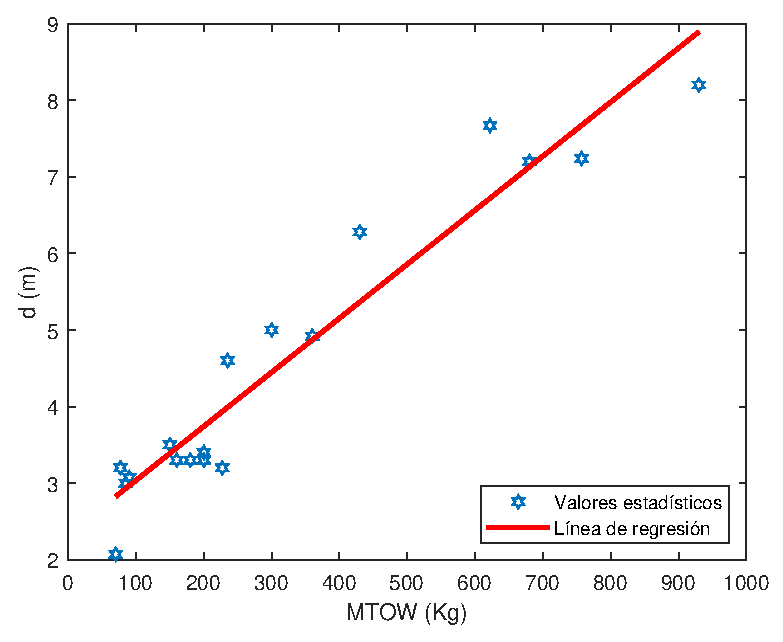
\includegraphics[width=80mm]{graficos/anald}
	\caption{Relación entre los diámetros de las palas de los helicópteros y sus MTOW}
\end{figure}
\begin{figure}
	\centering
	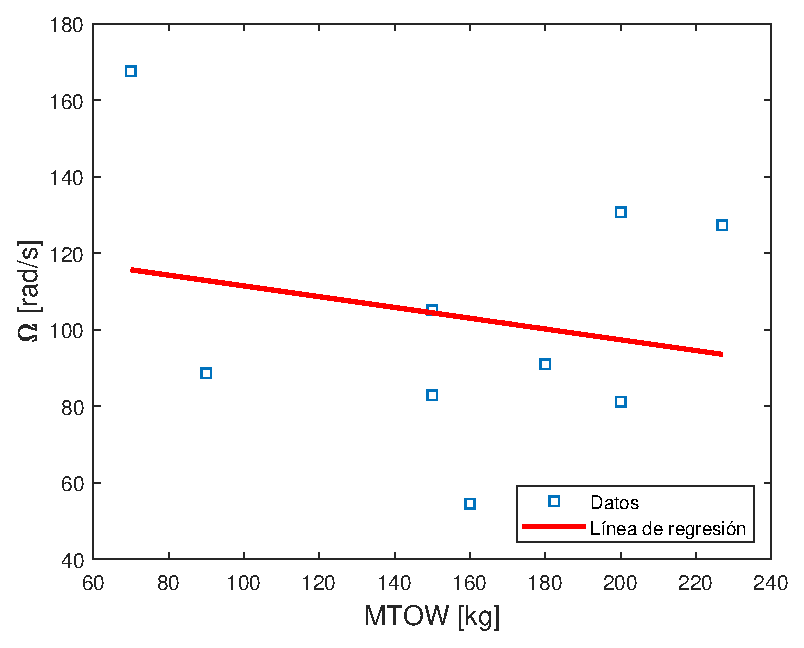
\includegraphics[width=80mm]{graficos/analomega}
	\caption{Relación entre las velocidades de giro del rotor de los helicópteros y sus MTOW}
\end{figure}
\begin{figure}
	\centering
	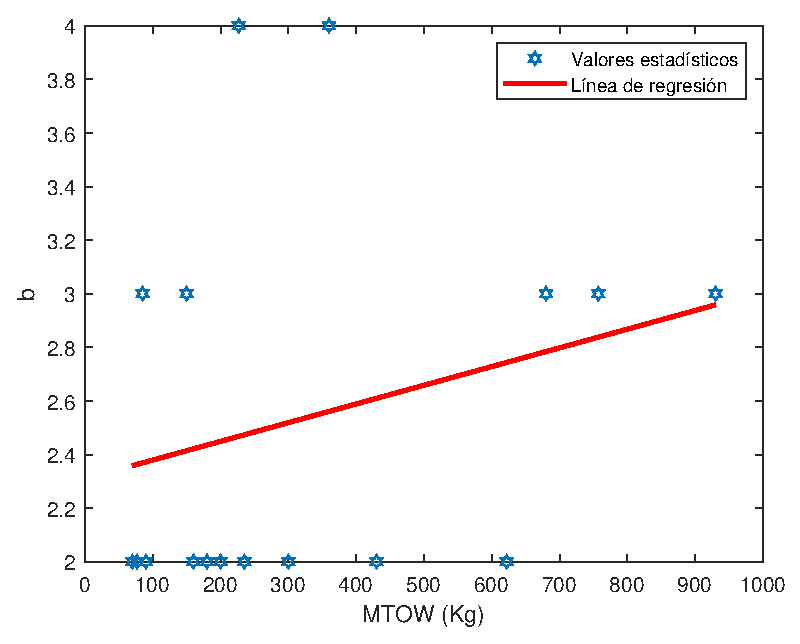
\includegraphics[width=80mm]{graficos/analb}
	\caption{Relación entre el número de palas del rotor principal de los helicópteros y sus MTOW}
\end{figure}
\begin{figure}
	\centering
	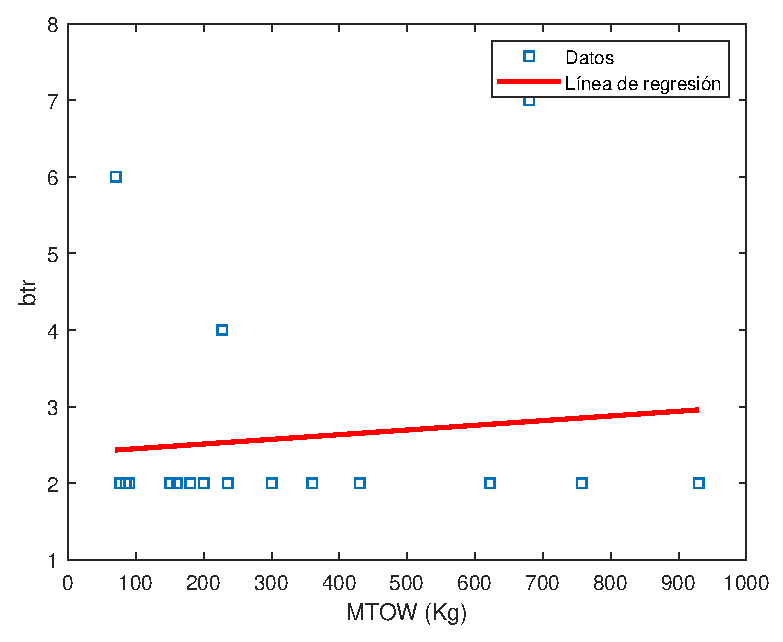
\includegraphics[width=80mm]{graficos/analbtr}
	\caption{Relación entre el número de palas del rotor antipar de los helicópteros y sus MTOW}
\end{figure}
\begin{figure}
	\centering
	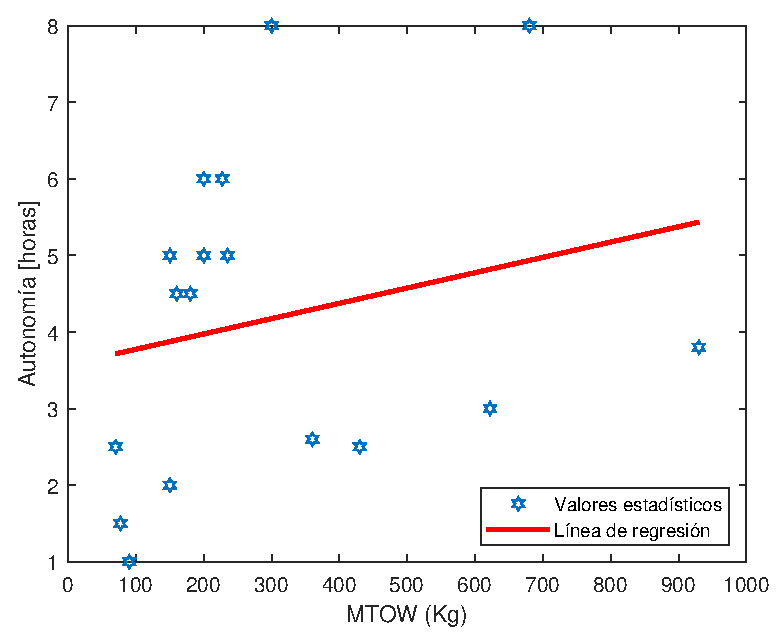
\includegraphics[width=80mm]{graficos/analaut}
	\caption{Relación entre las autonomías de los helicópteros y sus MTOW}
\end{figure}
\begin{figure}
	\centering
	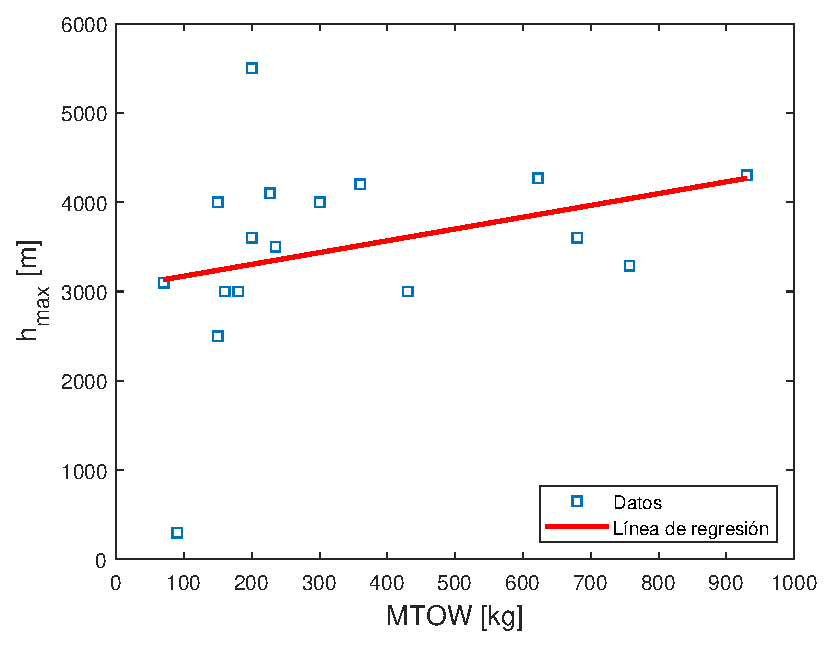
\includegraphics[width=80mm]{graficos/analtecho}
	\caption{Relación entre los techos de vuelo de los helicópteros y sus MTOW}
\end{figure}
\begin{figure}
	\centering
	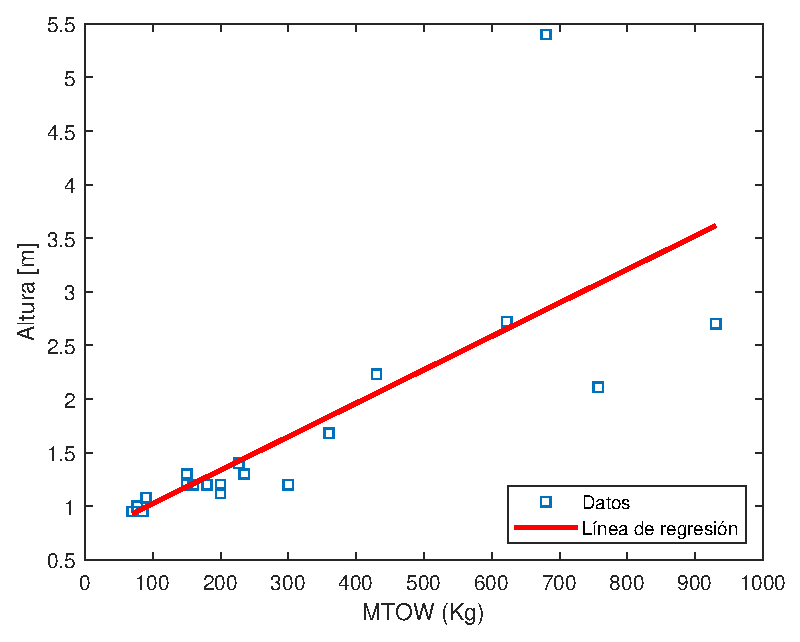
\includegraphics[width=80mm]{graficos/analalt}
	\caption{Relación entre las alturas de los helicópteros y sus MTOW}
\end{figure}
\begin{figure}
	\centering
	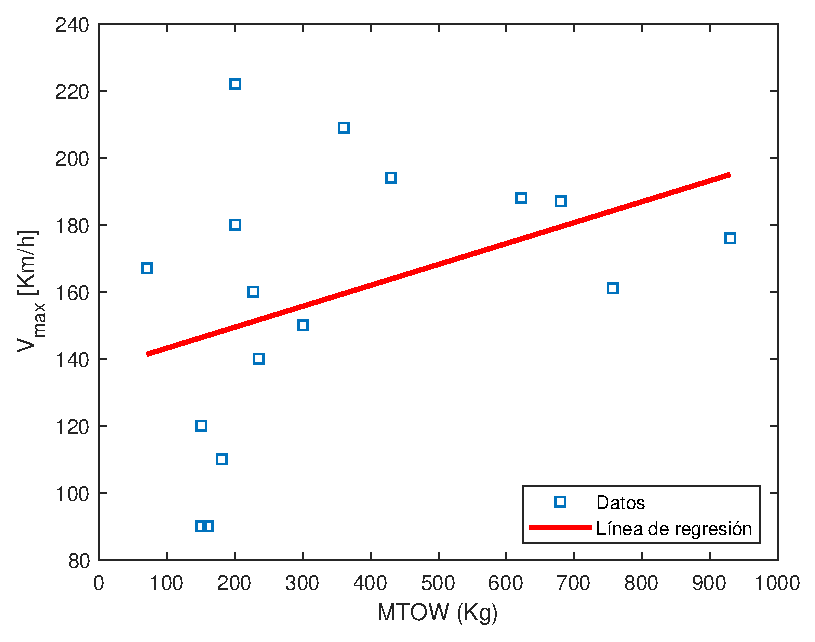
\includegraphics[width=80mm]{graficos/analv}
	\caption{Relación entre las velocidades máximas de avance de los helicópteros y sus MTOW}
\end{figure}
